\documentclass[a4paper, 14pt]{extarticle}

% Поля
%--------------------------------------
\usepackage{geometry}
\geometry{a4paper,tmargin=2cm,bmargin=2cm,lmargin=3cm,rmargin=1cm}
%--------------------------------------

\usepackage{float}
%Russian-specific packages
%--------------------------------------
\usepackage[T2A]{fontenc}
\usepackage[utf8]{inputenc} 
\usepackage[english, main=russian]{babel}
%--------------------------------------

\usepackage{textcomp}
\usepackage{xcolor}

% Красная строка
%--------------------------------------
\usepackage{indentfirst}               
%--------------------------------------
%Листинги
%--------------------------------------
\usepackage{listings}
\lstset{
  basicstyle=\ttfamily\footnotesize,
  breakatwhitespace=false,
  breaklines=true,
  captionpos=t,
  inputencoding=utf8,
  extendedchars=true,
  literate={а}{а}1{б}{б}1{в}{в}1{г}{г}1{д}{д}1{е}{е}1{ё}{ё}1{ж}{ж}1{з}{з}1{и}{и}1{й}{й}1{к}{к}1{л}{л}1{м}{м}1{н}{н}1{о}{о}1{п}{п}1{р}{р}1{с}{с}1{т}{т}1{у}{у}1{ф}{ф}1{х}{х}1{ц}{ц}1{ч}{ч}1{ш}{ш}1{щ}{щ}1{ъ}{ъ}1{ы}{ы}1{ь}{ь}1{э}{э}1{ю}{ю}1{я}{я}1,
  frame=single,
  keepspaces=true,
  keywordstyle=\bf,
  numbers=none,
  xleftmargin=25pt,
  xrightmargin=25pt,
  showspaces=false,
  showstringspaces=false,
  showtabs=false,
  stepnumber=1,
  tabsize=2,
  title=\lstname
}
%--------------------------------------
\usepackage[most]{tcolorbox}
\tcbuselibrary{listings,breakable}
\newtcblisting{breakablelisting}{
  listing only,
  breakable,
  enhanced,
  frame hidden,
  colback=white,
  left=8pt,
  overlay={\draw[line width=0.4pt] (frame.north west) -- (frame.south west);
          \draw[line width=0.4pt] ([xshift=3pt]frame.north west) -- ([xshift=3pt]frame.south west);},
  listing options={
    frame=none,
    numbers=none,
    mathescape=false,
    texcl=false,
    inputencoding=utf8,
    extendedchars=true,
    literate={а}{а}1{б}{б}1{в}{в}1{г}{г}1{д}{д}1{е}{е}1{ё}{ё}1{ж}{ж}1{з}{з}1{и}{и}1{й}{й}1{к}{к}1{л}{л}1{м}{м}1{н}{н}1{о}{о}1{п}{п}1{р}{р}1{с}{с}1{т}{т}1{у}{у}1{ф}{ф}1{х}{х}1{ц}{ц}1{ч}{ч}1{ш}{ш}1{щ}{щ}1{ъ}{ъ}1{ы}{ы}1{ь}{ь}1{э}{э}1{ю}{ю}1{я}{я}1,
    literate={\$}{{\$}}1
  }
}


%Graphics
%--------------------------------------
\usepackage{graphicx}
\usepackage{wrapfig}
%--------------------------------------
\graphicspath{{./lab5/}{./}}
% Полуторный интервал
%--------------------------------------
\linespread{1.3}                    
%--------------------------------------

%Выравнивание и переносы
%--------------------------------------
% Избавляемся от переполнений
\sloppy
% Запрещаем разрыв страницы после первой строки абзаца
\clubpenalty=10000
% Запрещаем разрыв страницы после последней строки абзаца
\widowpenalty=10000
%--------------------------------------

%Списки
\usepackage{enumitem}

%Подписи
\usepackage{caption} 

%Гиперссылки
\usepackage{hyperref}

\hypersetup {
	unicode=true
}

%Рисунки
%--------------------------------------
\DeclareCaptionLabelSeparator*{emdash}{~--- }
\captionsetup[figure]{labelsep=emdash,font=onehalfspacing,position=bottom}
%--------------------------------------

\usepackage{tempora}

%--------------------------------------

%%% Математические пакеты %%%
%--------------------------------------
\usepackage{amsthm,amsfonts,amsmath,amssymb,amscd}  % Математические дополнения от AMS
\usepackage{mathtools}                              % Добавляет окружение multlined
\usepackage[perpage]{footmisc}
%--------------------------------------

%--------------------------------------
%			НАЧАЛО ДОКУМЕНТА
%--------------------------------------

\begin{document}

%--------------------------------------
%			ТИТУЛЬНЫЙ ЛИСТ
%--------------------------------------
\begin{titlepage}
\thispagestyle{empty}
\newpage


%Шапка титульного листа
%--------------------------------------
\vspace*{-60pt}
\hspace{-65pt}
\begin{minipage}{0.3\textwidth}
\hspace*{-20pt}\centering
\includegraphics[width=\textwidth]{emblem}
\end{minipage}
\begin{minipage}{0.67\textwidth}\small \textbf{
\vspace*{-0.7ex}
\hspace*{-6pt}\centerline{Министерство науки и высшего образования Российской Федерации}
\vspace*{-0.7ex}
\centerline{Федеральное государственное автономное образовательное учреждение }
\vspace*{-0.7ex}
\centerline{высшего образования}
\vspace*{-0.7ex}
\centerline{<<Московский государственный технический университет}
\vspace*{-0.7ex}
\centerline{имени Н.Э. Баумана}
\vspace*{-0.7ex}
\centerline{(национальный исследовательский университет)>>}
\vspace*{-0.7ex}
\centerline{(МГТУ им. Н.Э. Баумана)}}
\end{minipage}
%--------------------------------------

%Полосы
%--------------------------------------
\vspace{-25pt}
\hspace{-35pt}\rule{\textwidth}{2.3pt}

\vspace*{-20.3pt}
\hspace{-35pt}\rule{\textwidth}{0.4pt}
%--------------------------------------

\vspace{1.5ex}
\hspace{-35pt} \noindent \small ФАКУЛЬТЕТ\hspace{80pt} <<Информатика и системы управления>>

\vspace*{-16pt}
\hspace{47pt}\rule{0.83\textwidth}{0.4pt}

\vspace{0.5ex}
\hspace{-35pt} \noindent \small КАФЕДРА\hspace{50pt} <<Теоретическая информатика и компьютерные технологии>>

\vspace*{-16pt}
\hspace{30pt}\rule{0.866\textwidth}{0.4pt}
  
\vspace{11em}

\begin{center}
\Large {\bf Лабораторная работа №2} \\ 
\large {\bf по курсу <<Моделирование>>} \\
\large <<Оценивание функций связи между ненаблюдаемыми одновременно параметрами>> 
\end{center}\normalsize

\vspace{8em}


\begin{flushright}
  {Студент группы ИУ9-82Б Шемякин В.А. \hspace*{15pt}\\ 
  \vspace{2ex}
  Преподаватель Домрачева А.Б.\hspace*{15pt}}
\end{flushright}

\bigskip

\vfill
 

\begin{center}
\textsl{Москва 2026}
\end{center}
\end{titlepage}
%--------------------------------------
%		КОНЕЦ ТИТУЛЬНОГО ЛИСТА
%--------------------------------------

\renewcommand{\ttdefault}{pcr}

\setlength{\tabcolsep}{3pt}
\newpage
\setcounter{page}{2}
\section{Постановка задачи}

Пусть имеются две выборки значений случайной величины, полученные при различных состояниях системы, при этом прямое соответствие между отдельными наблюдениями отсутствует. Предполагается, что существует некоторая монотонная функция связи, преобразующая значения первой случайной величины в значения второй. Требуется на основе статистических данных построить математическую модель такой функции связи.

В качестве исходных данных используются две выборки значений параметра~--- уровня глюкозы~--- соответствующие различным состояниям наблюдаемого объекта. Поскольку значения параметров не наблюдаются попарно, задача решается путём сопоставления эмпирических распределений этих выборок. Необходимо оценить параметры модели функции преобразования вида $\varphi(x) = \alpha x^{\beta}$, которая позволяет преобразовать значения первой выборки таким образом, чтобы распределение преобразованных данных было максимально близко к распределению второй выборки.

Целью лабораторной работы является построение математической модели функции связи между двумя случайными параметрами, не наблюдаемыми одновременно, на основе анализа их статистических распределений.

\section{Построение математической модели}

Входные данные содержат записи пациентов с пятью числовыми параметрами. Используется столбец, содержащий уровень глюкозы, и столбец, указывающий наличие диабета (0 или 1).

Обозначим через $\xi_0$ выборку уровня глюкозы для пациентов без диабета (Outcome = 0) и через $\xi_1$ выборку для пациентов с диабетом (Outcome = 1). Каждая выборка состоит из упорядоченных по возрастанию значений.

Предлагается модель преобразования выборки $\xi_0$ в выборку, близкую по распределению к $\xi_1$, через функцию $\varphi(x) = \alpha x^{\beta}$, где $\alpha > 0$ и $\beta > 0$. Параметры модели $\alpha$ и $\beta$ оцениваются методом моментов. Для каждого элемента выборки $x_i \in \xi_0$ вычисляется преобразованное значение $\varphi(x_i) = \alpha x_i^{\beta}$.

Качество модели оценивается по максимальному расстоянию между эмпирическими функциями распределения. Пусть $F_0(z)$~--- эмпирическая функция распределения выборки $\xi_0$, $F_1(z)$~--- эмпирическая функция распределения выборки $\xi_1$, и $F_\varphi(z)$~--- эмпирическая функция распределения преобразованной выборки $\varphi(\xi_0)$. Критерий согласия определяется как:
\begin{equation}
D = \max_z \left| F_\varphi(z) - F_1(z) \right|.
\end{equation}
Чем меньше значение $D$, тем лучше преобразованная выборка соответствует целевому распределению.

Модель устроена следующим образом. На вход подаются две выборки $\xi_0$ и $\xi_1$, полученные при различных состояниях системы. По обеим выборкам методом моментов оцениваются параметры $\alpha$ и $\beta$. Затем к каждому элементу выборки $\xi_0$ применяется степенное преобразование $\varphi(x) = \alpha x^{\beta}$, в результате чего формируется преобразованная выборка $\varphi(\xi_0)$. После этого эмпирическая функция распределения преобразованной выборки сравнивается с эмпирической функцией распределения целевой выборки $\xi_1$ по критерию максимального расхождения. Схема модели представлена на рисунке~\ref{fig:model}.

\begin{figure}[H]
  \centering
  
\includegraphics[width=0.8\textwidth]{Lab4/screen1.jpg}
  \caption{Схема модели преобразования выборок}
  \label{fig:model}
\end{figure}

\section{Решение вычислительной задачи}

\subsection{Оценка параметров модели}

Для оценки параметров $\alpha$ и $\beta$ применяется метод моментов. Предполагается, что преобразованная выборка $\varphi(\xi_0)$ имеет распределение, близкое к распределению $\xi_1$, поэтому приравниваются первые и вторые моменты:
\begin{equation}
M[\ln(\xi_1)] = M[\ln(\varphi(\xi_0))], \quad D[\ln(\xi_1)] = D[\ln(\varphi(\xi_0))],
\end{equation}
где $M[\cdot]$ обозначает математическое ожидание, а $D[\cdot]$~--- дисперсию (выборочную, несмещённую).

Из этих условий получается система:
\begin{equation}
\begin{cases}
\overline{\ln \xi_1} = \ln\alpha + \beta \cdot \overline{\ln \xi_0}, \\[4pt]
D[\ln \xi_1] = \beta^2 \cdot D[\ln \xi_0],
\end{cases}
\end{equation}
где $\overline{\ln \xi_k} = \dfrac{1}{n_k}\displaystyle\sum_{i=1}^{n_k} \ln \xi_k^{(i)}$~--- выборочное среднее логарифмов, а $D[\ln \xi_k] = \dfrac{1}{n_k - 1}\displaystyle\sum_{i=1}^{n_k}\bigl(\ln\xi_k^{(i)} - \overline{\ln \xi_k}\bigr)^2$~--- несмещённая выборочная дисперсия.

Из второго уравнения системы находим $\beta$, из первого~--- $\alpha$:
\begin{equation}
\hat\beta = \sqrt{\frac{D[\ln(\xi_1)]}{D[\ln(\xi_0)]}}, \quad \hat\alpha = \exp\!\left(\overline{\ln\xi_1} - \hat\beta \cdot \overline{\ln\xi_0}\right).
\end{equation}

\subsection{Оценка эффективности модели}

Для оценки эффективности модели вычисляется максимальное расстояние между эмпирическими функциями распределения до и после преобразования. Пусть:
\begin{equation}
D_0 = \max_z \left| F_0(z) - F_1(z) \right|
\end{equation}
характеризует исходное расхождение между распределениями выборок $\xi_0$ и $\xi_1$, а
\begin{equation}
D_{\text{модели}} = \max_z \left| F_\varphi(z) - F_1(z) \right|
\end{equation}
характеризует расхождение после применения преобразования. Отношение $D_0 / D_{\text{модели}}$ показывает, во сколько раз модель уменьшает расстояние между распределениями, и служит мерой эффективности преобразования.

\section{Анализ модели}

Для получения объективной оценки качества модели исходные данные разделяются на две части: рабочую выборку для оценки параметров и контрольную выборку для проверки качества. Параметры модели оцениваются только на рабочей части, что исключает смещение оценок и позволяет объективно оценить обобщающую способность модели. Тестирование проводилось с двумя вариантами разделения: 80/20 (рабочая/контрольная) и 70/30.

При разделении 80\% (рабочая) на 20\% (контрольная) получены следующие результаты. Методом моментов на рабочей выборке оценены параметры: $\alpha = 1{,}273623$, $\beta = 1{,}002422$. На рабочей выборке исходное расстояние между распределениями групп составило $D_0^{\text{раб}} = 0{,}445951$, после применения преобразования расстояние сократилось до $D_{\text{модели}}^{\text{раб}} = 0{,}079630$. На контрольной выборке исходное расстояние составило $D_0^{\text{контр}} = 0{,}437778$, расстояние после преобразования $D_{\text{модели}}^{\text{контр}} = 0{,}075556$. Близость результатов на обеих выборках указывает на хорошую обобщающую способность модели.

При разделении 70\% (рабочая) на 30\% (контрольная) оценки параметров составили: $\alpha = 1{,}298326$, $\beta = 0{,}996923$. На рабочей выборке исходное расстояние составило $D_0^{\text{раб}} = 0{,}433020$, после преобразования $D_{\text{модели}}^{\text{раб}} = 0{,}084379$. На контрольной выборке исходное расстояние $D_0^{\text{контр}} = 0{,}461667$, расстояние после преобразования $D_{\text{модели}}^{\text{контр}} = 0{,}095000$. 

Сравнение двух вариантов показывает, что оба разделения дают близкие результаты с показателем степени $\beta$ близким к единице, что указывает на стабильность полученных оценок и примерно линейную связь между уровнями глюкозы в двух группах. Близость значений $D_{\text{модели}}$ на рабочей и контрольной выборках подтверждает надёжность модели и отсутствие переобучения.

На рисунке~\ref{fig:before} приведены функции распределения уровня глюкозы в исходных выборках. На рисунке~\ref{fig:after} показаны функции распределения преобразованной выборки и целевой выборки.

\begin{figure}[H]
  \centering
  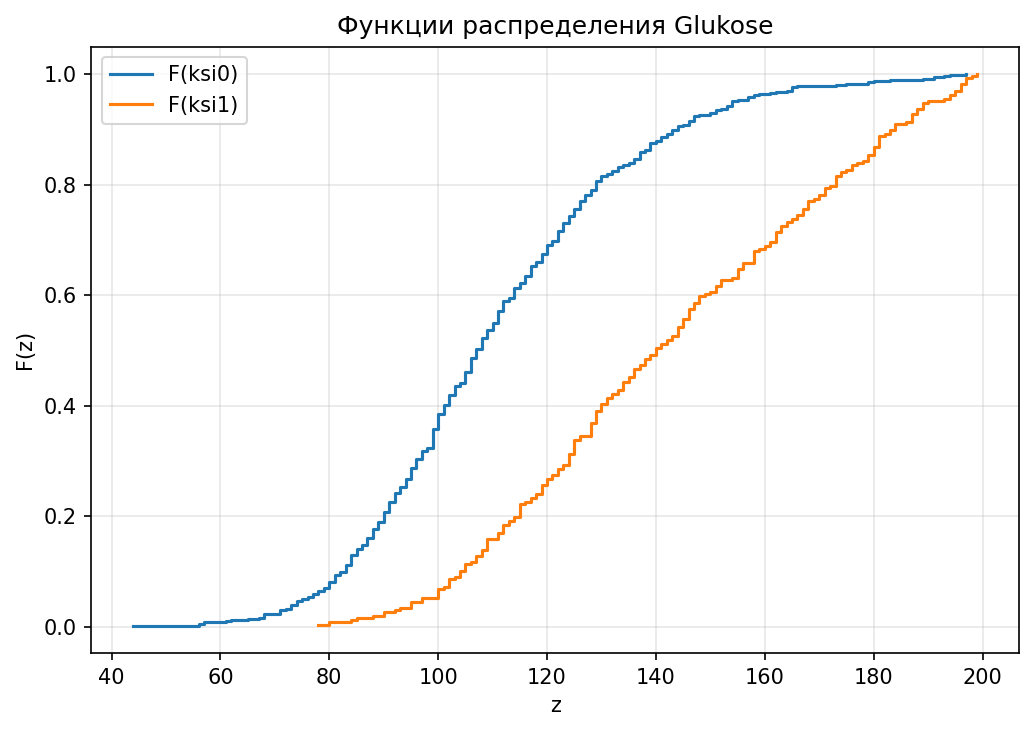
\includegraphics[width=0.8\textwidth]{glucose_distribution.png}
  \caption{Функции распределения уровня глюкозы для пациентов без диабета и с диабетом}
  \label{fig:before}
\end{figure}

\begin{figure}[H]
  \centering
  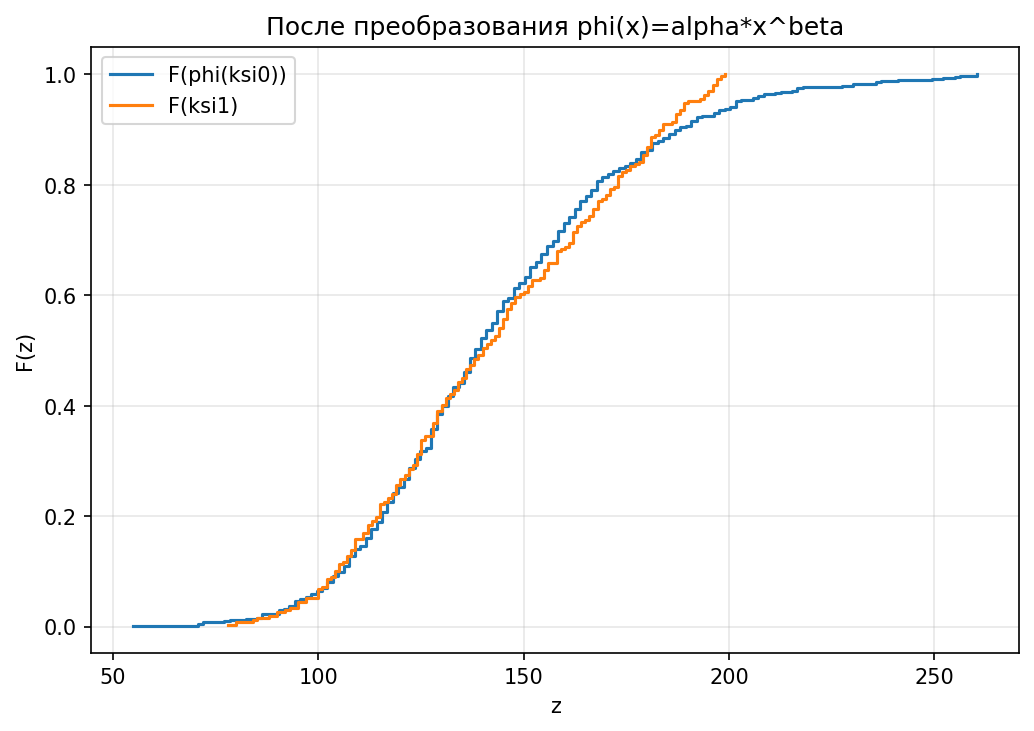
\includegraphics[width=0.8\textwidth]{glucose_transformed_distribution.png}
  \caption{Функции распределения после преобразования $\varphi(x) = \alpha x^{\beta}$ и целевой выборки}
  \label{fig:after}
\end{figure}

Полученные результаты в обоих вариантах разделения свидетельствуют об устойчивости модели.

\section{Вывод}

В ходе данной лабораторной работы была построена математическая модель для установления функциональной связи между уровнем глюкозы в группах пациентов с диабетом и без диабета. Модель основана на степенном преобразовании вида $\varphi(x) = \alpha x^{\beta}$, где параметры оценены методом моментов на рабочей выборке. Проведена проверка модели с использованием двух вариантов разделения данных (80/20 и 70/30), и оценка качества выполнена на обеих выборках с использованием критерия максимального расхождения эмпирических функций распределения. Результаты показывают, что расстояние между распределениями на контрольной выборке сопоставимо с расстоянием на рабочей, что подтверждает надёжность метода.

\section{Практическая реализация}

\refstepcounter{lstlisting}\label{lst:code}
\noindent Листинг~\ref{lst:code}. Исходный код программы.

\begin{breakablelisting}
import matplotlib
matplotlib.use('Agg')
import matplotlib.pyplot as plt
import numpy as np
import pandas as pd

RANDOM_SEED = 42


def load_samples(file_path):
    data = pd.read_csv(file_path, usecols=["Glucose", "Outcome"])
    data = data[data["Glucose"] > 0].copy()
    ksi0 = data.loc[data["Outcome"] == 0, "Glucose"].to_numpy(dtype=float)
    ksi1 = data.loc[data["Outcome"] == 1, "Glucose"].to_numpy(dtype=float)
    return ksi0, ksi1


def split_sample(sample, train_ratio=0.8, seed=None):
    if seed is not None:
        np.random.seed(seed)
    indices = np.arange(len(sample))
    np.random.shuffle(indices)
    split_point = int(len(sample) * train_ratio)
    train_indices = indices[:split_point]
    test_indices = indices[split_point:]
    return sample[train_indices], sample[test_indices]


def empirical_distribution(sample):
    sample = np.sort(np.asarray(sample, dtype=float))
    F = np.arange(1, len(sample) + 1) / len(sample)
    return sample, F


def max_distribution_difference(sample_1, sample_2):
    sample_1 = np.sort(np.asarray(sample_1, dtype=float))
    sample_2 = np.sort(np.asarray(sample_2, dtype=float))
    z = np.sort(np.unique(np.concatenate([sample_1, sample_2])))
    F1 = np.searchsorted(sample_1, z, side="right") / len(sample_1)
    F2 = np.searchsorted(sample_2, z, side="right") / len(sample_2)
    diff = np.abs(F1 - F2)
    i = np.argmax(diff)
    return diff[i], z[i]


def estimate_alpha_beta(ksi0, ksi1):
    lnx = np.log(ksi0)
    lny = np.log(ksi1)
    mean_x = np.mean(lnx)
    mean_y = np.mean(lny)
    var_x = np.var(lnx, ddof=1)
    var_y = np.var(lny, ddof=1)
    beta = np.sqrt(var_y / var_x)
    alpha = np.exp(mean_y - beta * mean_x)
    return alpha, beta, mean_y, mean_x, var_y, var_x


def phi(x, alpha, beta):
    return alpha * x**beta


def trim_tails(sample, low_q, high_q):
    sample = np.asarray(sample, dtype=float)
    if low_q <= 0 and high_q >= 1:
        return sample
    lo = np.quantile(sample, low_q)
    hi = np.quantile(sample, high_q)
    trimmed = sample[(sample >= lo) & (sample <= hi)]
    return trimmed


def save_distribution_plots(ksi0, ksi1, alpha, beta, d_raw, d_model):
    x0, F0 = empirical_distribution(ksi0)
    x1, F1 = empirical_distribution(ksi1)
    phi_x0, F_phi = empirical_distribution(phi(ksi0, alpha, beta))

    fig, ax = plt.subplots(figsize=(7, 5))
    ax.step(x0, F0, where="post", label="F(ksi0)")
    ax.step(x1, F1, where="post", label="F(ksi1)")
    ax.set_title(f"Функции распределения Glukose")
    ax.set_xlabel("z")
    ax.set_ylabel("F(z)")
    ax.grid(True, alpha=0.3)
    ax.legend()
    fig.tight_layout()
    fig.savefig("glucose_distribution.png", dpi=150, bbox_inches="tight")
    plt.close(fig)

    fig, ax = plt.subplots(figsize=(7, 5))
    ax.step(phi_x0, F_phi, where="post", label="F(phi(ksi0))")
    ax.step(x1, F1, where="post", label="F(ksi1)")
    ax.set_title(f"После преобразования phi(x)=alpha*x^beta")
    ax.set_xlabel("z")
    ax.set_ylabel("F(z)")
    ax.grid(True, alpha=0.3)
    ax.legend()
    fig.tight_layout()
    fig.savefig("glucose_transformed_distribution.png", dpi=150, bbox_inches="tight")
    plt.close(fig)


def print_results(alpha, beta, d_raw, z_raw, d_model, z_model):
    print(f"alpha = {alpha:.6f}")
    print(f"beta = {beta:.6f}")
    print(f"max|F(ksi0) - F(ksi1)| = {d_raw:.6f}, z = {z_raw:.6f}")
    print(f"max|F(phi(ksi0)) - F(ksi1)| = {d_model:.6f}, z = {z_model:.6f}")


def print_train_test_results(alpha, beta, d_raw_train, z_raw_train, d_model_train, z_model_train,
                              d_raw_test, z_raw_test, d_model_test, z_model_test):
    print(f"alpha = {alpha:.6f}")
    print(f"beta = {beta:.6f}")
    print(f"\nРабочая выборка:")
    print(f"  max|F(ksi0) - F(ksi1)| = {d_raw_train:.6f}, z = {z_raw_train:.6f}")
    print(f"  max|F(phi(ksi0)) - F(ksi1)| = {d_model_train:.6f}, z = {z_model_train:.6f}")
    if d_model_train > 0:
        improvement_train = d_raw_train / d_model_train
        print(f"  Улучшение: {improvement_train:.2f}x")
    print(f"\nКонтрольная выборка:")
    print(f"  max|F(ksi0) - F(ksi1)| = {d_raw_test:.6f}, z = {z_raw_test:.6f}")
    print(f"  max|F(phi(ksi0)) - F(ksi1)| = {d_model_test:.6f}, z = {z_model_test:.6f}")
    if d_model_test > 0:
        improvement_test = d_raw_test / d_model_test
        print(f"  Улучшение: {improvement_test:.2f}x")


def test_model(ksi0, ksi1, train_ratio, seed=None):
    ksi0_train, ksi0_test = split_sample(ksi0, train_ratio, seed)
    ksi1_train, ksi1_test = split_sample(ksi1, train_ratio, seed)
    
    alpha, beta, _, _, _, _ = estimate_alpha_beta(ksi0_train, ksi1_train)
    
    d_raw_train, z_raw_train = max_distribution_difference(ksi0_train, ksi1_train)
    d_model_train, z_model_train = max_distribution_difference(phi(ksi0_train, alpha, beta), ksi1_train)
    
    d_raw_test, z_raw_test = max_distribution_difference(ksi0_test, ksi1_test)
    d_model_test, z_model_test = max_distribution_difference(phi(ksi0_test, alpha, beta), ksi1_test)
    
    return alpha, beta, d_raw_train, z_raw_train, d_model_train, z_model_train, d_raw_test, z_raw_test, d_model_test, z_model_test


def main():
    ksi0, ksi1 = load_samples("diabetes.csv")
    
    print("=== Разделение 80 (рабочая) / 20 (контрольная) ===")
    alpha_80, beta_80, d_raw_train_80, z_raw_train_80, d_model_train_80, z_model_train_80, d_raw_test_80, z_raw_test_80, d_model_test_80, z_model_test_80 = test_model(ksi0, ksi1, 0.8, RANDOM_SEED)
    print_train_test_results(alpha_80, beta_80, d_raw_train_80, z_raw_train_80, d_model_train_80, z_model_train_80, d_raw_test_80, z_raw_test_80, d_model_test_80, z_model_test_80)
    
    print("\n=== Разделение 70 (рабочая) / 30 (контрольная) ===")
    alpha_70, beta_70, d_raw_train_70, z_raw_train_70, d_model_train_70, z_model_train_70, d_raw_test_70, z_raw_test_70, d_model_test_70, z_model_test_70 = test_model(ksi0, ksi1, 0.7, RANDOM_SEED)
    print_train_test_results(alpha_70, beta_70, d_raw_train_70, z_raw_train_70, d_model_train_70, z_model_train_70, d_raw_test_70, z_raw_test_70, d_model_test_70, z_model_test_70)


if __name__ == "__main__":
    main()
\end{breakablelisting}

\end{document}